% !TeX encoding = UTF-8
% !TeX root = V26_Halleffekt.tex
% !TeX spellcheck = de_DE_frami

\section{Durchführung}
Wir untersuchen im Folgenden eine $d = 0,31\,\micro\metre$ dünne Schicht aus Bor-dotiertem Silizium, die auf einem Wafer aufgetragen wurde. Da \textsf{B} 3 Valenzelektronen besitzt, \textsf{Si} aber 4, können diese Löcher im sonst vierbindigen Kristallgitter in das Valenzband übergehen -- der Halbleiter ist folglich p-dotiert.

Anstatt die Kontaktstellen klein zu halten, vermessen wir eine Probe in stilisierter Kleeblatt-Form (vier radialen Einkerbungen, vgl. Abbildung \ref{fig:probe}). Durch die höhere Stromdichte im Zentrum dominiert dieses die elektrischen Eigenschaften der Probe, wodurch auf den vier \glqq Blättern\grqq{} relativ große Kontakte platziert werden können, ohne die Messung zu stören. Zudem sind die Abstände zweier Kontakte relativ scharf definiert, da der Strom immer über die Mitte fließt.

Bevor die Probe vermessen werden kann, muss allerdings das Magnetfeld und die Ausrichtung der Probe zu diesem kalibriert werden; die Berechnung geht von einem senkrecht zur Probe angelegten Feld aus. Weiterhin wird geprüft, ob die Probenkontakte bei den verwendeten Strömen noch als ohmsch angenommen werden können.

\begin{figure}[p]
\centering
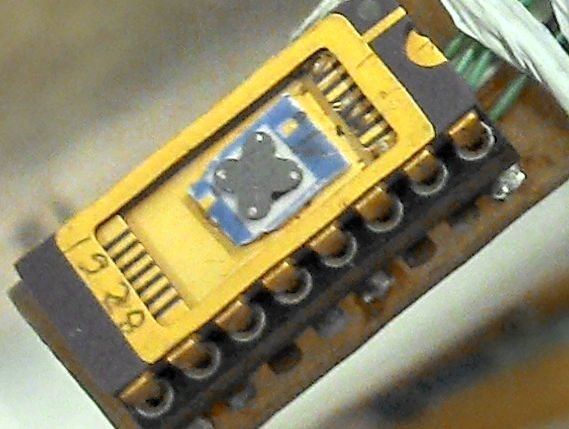
\includegraphics[width=0.3\textwidth]{trefoil.jpg}
\caption{Foto der Probe in stilisierter Kleeblatt-Form.}
\label{fig:probe}
\end{figure}

\subsection{Vorbereitung}
An den Probenhalter wird anstelle des \textsf{Si}-Scheibchens ein Hall-Sensor mit bekannter Hall-Konstante angebracht, der mit $I_H = 100\,$mA versorgt wird. Für diese Konfiguration gilt $B = 0,01172 \,\tfrac{\tesla}{\milli\volt} \cdt U_H$, wobei $U_H$ die am Sensor gemessene Hallspannung ist.\\[1ex]
Der Spulenstrom $I_M$ des Magneten wird nun in 1\,A-Schritten bis auf 15\,A hochgefahren. Für die folgenden Versuche wird der Strom eingestellt, für den wir $B \approx 0,5 \,\tesla$ erzielen.

Nun wird die Hallsonde durch unsere Probe ersetzt. Die $U$-$I$-Kennlinie zwischen zwei willkürlich gewählten Kontakten soll im Bereich $I \in [0,~150]\,\micro\ampere$ abgenommen werden. Abhängig von dem Material der Kontakte könnte der Übergangsbereich eine Schottky-Diode bilden, wodurch Ströme in Sperrrichtung geblockt würden. Da der Strom aber bei sämtlichen Messungen über gleichartige Kontakte zu- und abfließt, die ggf. zusammen in beide Richtung sperren würden, muss bei der Präparation der Probe ein Kontaktmaterial mit ohmschem Übergang gewählt worden sein.

Als letzte Vormessung drehen wir die Probe in 10\degree-Schritten von -90\degree bis +90\degree, um zu prüfen, ob diese wirklich senkrecht zum Magnetfeld ausgerichtet ist. Dabei messen wir die transversale Spannung $U_t$ bei $I_H = 100\,\micro\ampere$ und tragen diese gegen den Winkel auf.


\newpage
\subsection{Bestimmung von $\mu ~\&~ p$ über $\rho ~\&~ R_H$}
\enlargethispage{4em}

Da der Versuchsaufbau für Präzisionsmessungen ausgelegt ist, wird der von der Konstantstromquelle bereitgestellte Strom über eine Stromsenke abgeführt. Diese ermöglicht eine genauere Bestimmung des durch die Probe fließenden Stroms. Für die Messung der Spannungen genügt ein hochohmiges Voltmeter.

Die Apparatur der Firma Keithley nutzt eine Schalt-Matrix aus Relais (Abbildung \ref{fig:keithley3}), wodurch alle vier benachbarten Kontakt-Paare in beide Stromrichtungen beschaltet werden können. Somit ergeben sich 8 Mess-Konfigurationen für die Bestimmung des spezifischen Widerstands $\rho$.
Die Nummerierung der gemessenen Spannungen $V^R_1, \dots, V^R_8$ ist in Tabelle 3-3 der Versuchanleitung (Abbildung \ref{fig:keithley1}) ersichtlich.

Unter Kenntnis der Dicke $d$ des Plättchens, des Formfaktors $f \approx 1$ und des Stroms  $I = 100\,\micro\ampere$ erhält man\\[-1.2em]
\begin{equation}
\rho ~=~ 1,1331 \cdot \frac{f \cdt d}{2 \cdt I} ~ \sum\limits_{i=1}^8 (-1)^i \; V^R_i
\end{equation}

Da es nur zwei \glqq diagonale\grqq{} (gegenüberliegende) Verbindungen gibt, erhält man inklusive der Umpolung des Stroms 4 Beschaltungen für den Halleffekt. Während das Manual \cite{lit:manual} vorsieht, die Messung nach Umpolen des Magnetfeldes zu wiederholen, genügen  gemäß dem Reziprozitätstheorem für passive Vierpole bereits diese vier Messungen, um die Offset-Spannung aus Gleichung \eqref{eq:U_offset} zu eliminieren. Diese Vereinfachung reduziert den Aufwand für die Messung beträchtlich. Die Zuordnung von $V^H_1, \dots, V^H_4$ erfolgt gemäß Tabelle 3-4 der Anleitung (Abbildung \ref{fig:keithley2}).
% REZIPROZITÄTSTHEOREM FÜR PASSIVE VIERPOLE

Zieht man neben $d$ und $I$ (gleichbleibend zur vorherigen Messung) noch das zuvor eingestellte Magnetfeld $B$ hinzu, so ergibt sich für den Hallkoeffizienten 
\begin{equation}
R_H ~=~ \frac{0,25 \cdt d}{B \cdt I} ~ \sum\limits_{i=1}^4 (-1)^i \; V^H_i
\end{equation}
Da $R_H$ typischerweise in $\tfrac{\centi\metre^3}{\ampere\second}$, $d$ in cm und $B$ in T angegeben wird, ergibt sich in diesem Fall ein Vorfaktor von 2500 anstelle 0,25.

Die Beweglichkeit ergibt sich zu
\begin{equation}
\mu ~=~ \frac{|R_H|}{\rho}
\end{equation}
und mit Gleichung \eqref{eq:p_rho_mu} erhalten wir schließlich die Löcherkonzentration
\begin{equation}
p = (e \cdt R_H)^{-1}.
\end{equation}

Die Probe wird in einem Kryostat durch flüssigen Stickstoff auf 80\,K abgekühlt und anschließend durch einen Heizwiderstand langsam aufgewärmt, während alle 5\,K eine Messung gestartet wird. Bei 300\,K wird die Messreihe beendet.

\begin{figure}[p]
\centering
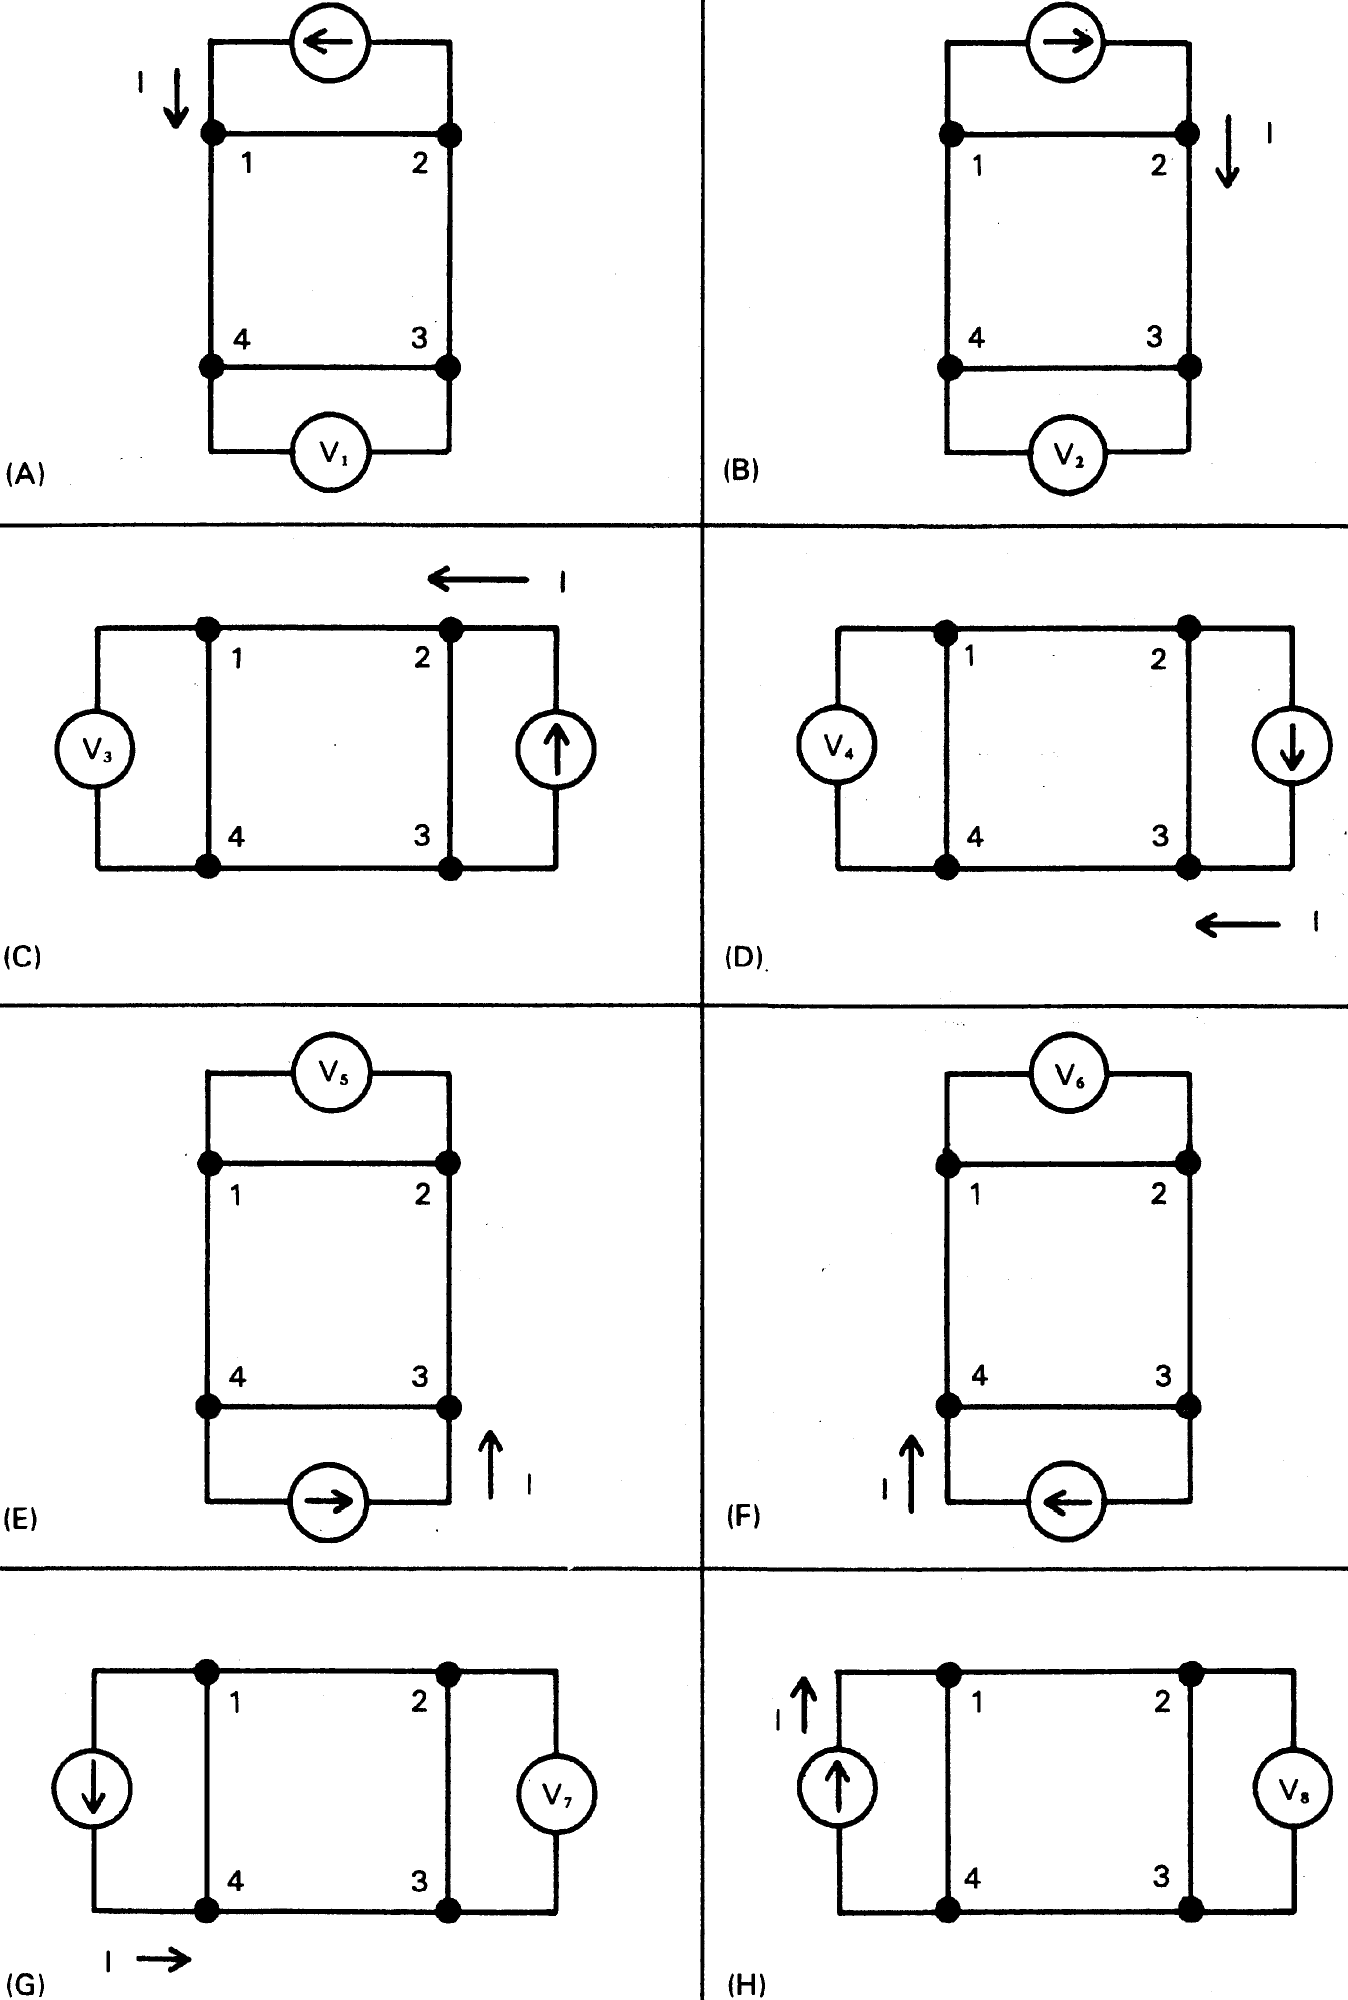
\includegraphics[width=0.7\textwidth]{Keithley_rho.png}
\caption{Messkonfigurationen für den spezifischen Widerstand $\rho$. \cite[Fig. 3-3]{lit:manual}}
\label{fig:keithley1}
\end{figure}

\begin{figure}[p]
\centering
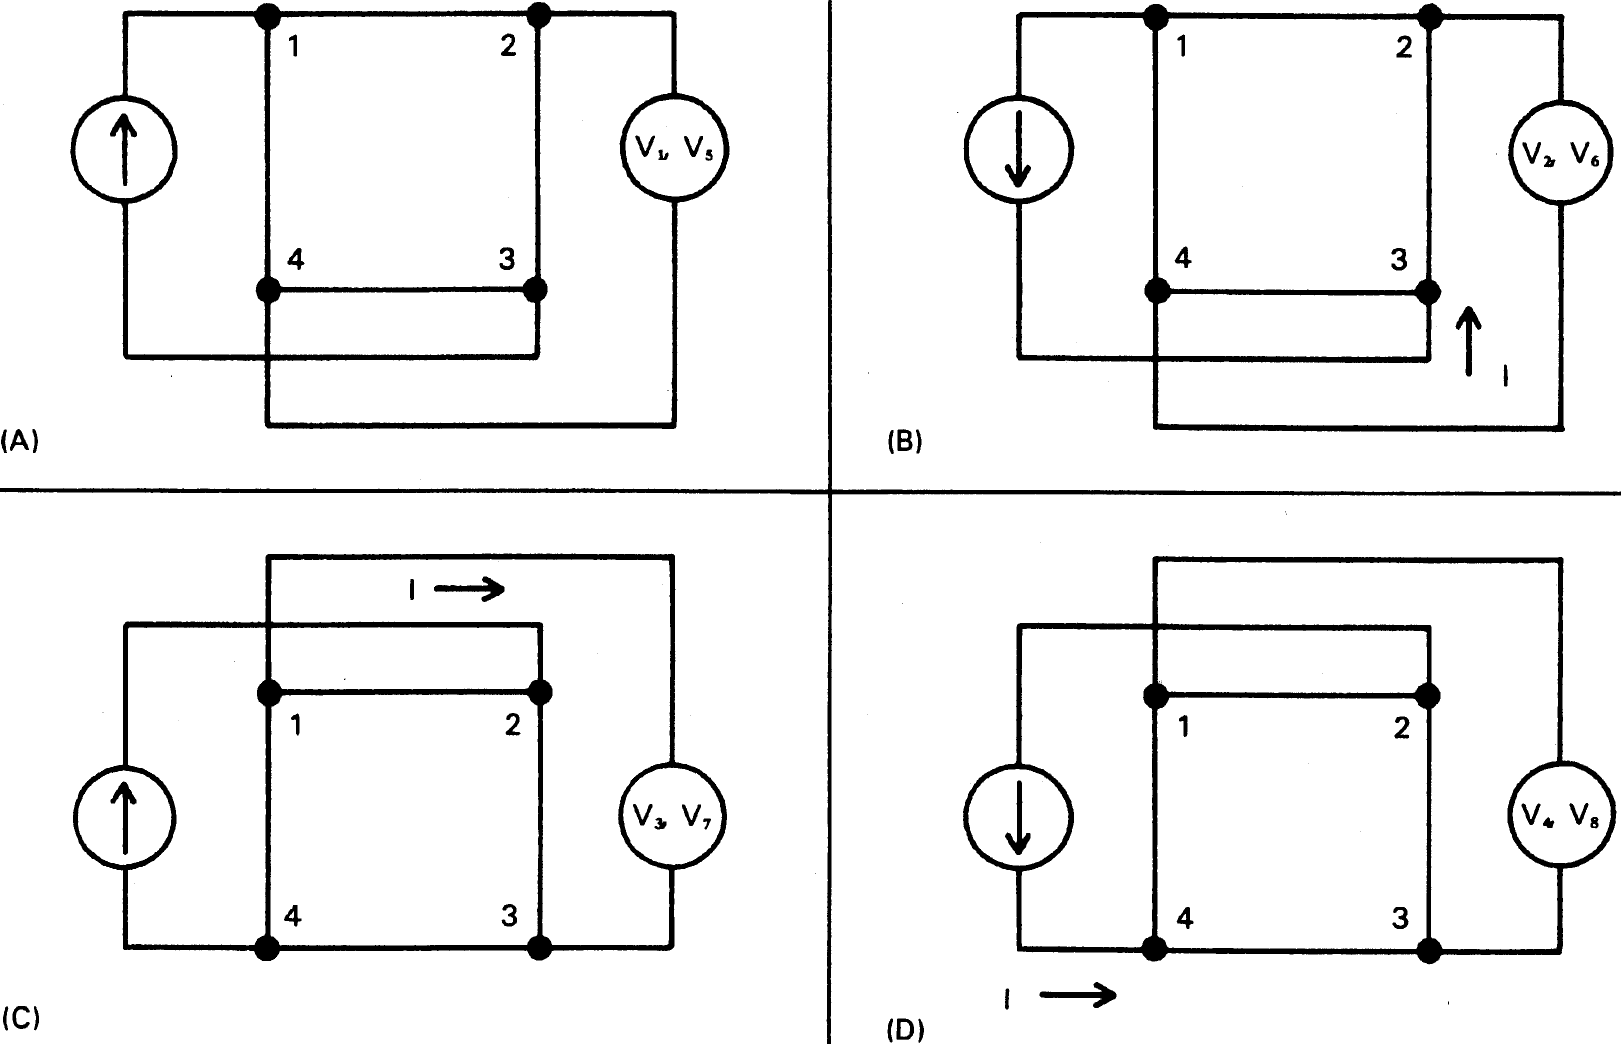
\includegraphics[width=0.7\textwidth]{Keithley_R_H.png}
\caption{Messkonfigurationen für die Hall-Konstante $R_H$. \cite[Fig. 3-4]{lit:manual}}
\label{fig:keithley2}
\end{figure}

\begin{figure}[p]
\centering
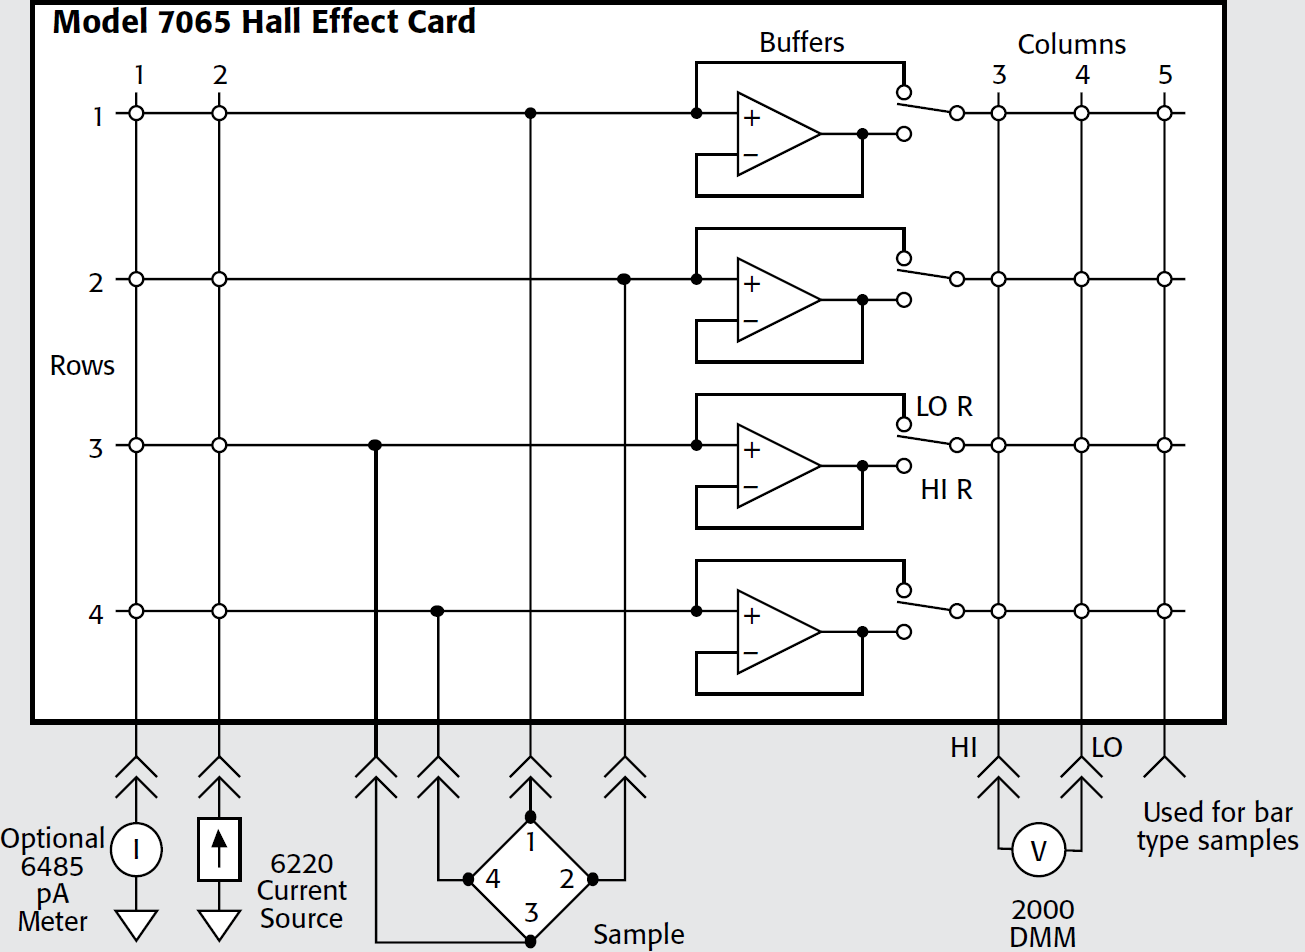
\includegraphics[width=0.9\textwidth]{Relais_new.png}
\caption{Schema der Messelektronik: Schaltmatrix und Messinstrumente. \cite{lit:keithley}}
\vspace{1ex}
Für die Widerstandsmessung werden Stromquelle (6220) und -senke (6485) an benachbarte Kontakte geschaltet, bei der Hall-Konfiguration an gegenüberliegende. Die verbleibenden Kontakte sind mit dem Voltmeter (2000) verschaltet. Die in die Schaltmatrix integrierten Puffer werden nur bei hochohmigen Proben zugeschaltet.
\label{fig:keithley3}
\end{figure}

\newpage
\section{Auswertung}

\subsection{Induktivität des Elektromagneten}
Die Messpunkte und Regression sind in Abbildung \ref{fig:plot_B} aufgetragen. Wie erwartet hängt die Magnetfeldstärke linear vom Strom ab.

Da wir die angestrebte Magnetfeldstärke von $B = 0,5 \,\tesla$ nicht genau erreichen müssen, wählen wir den nächstliegenden Datenpunkt: Bei 13\,A erzeugt der Elektromagnet ein Feld von 0,509\,T.

\begin{figure}[p]
\centering
% This file was created by matlab2tikz v0.5.0 (commit 240e05cc8ef02a03772d66c5a06ee6e5e3ffe2c8) running on MATLAB 8.2.
%Copyright (c) 2008--2014, Nico Schlömer <nico.schloemer@gmail.com>
%All rights reserved.
%Minimal pgfplots version: 1.3
%
\begin{tikzpicture}

\begin{axis}[%
width=0.95092\textwidth,
height=0.75\textwidth,
at={(0\textwidth,0\textwidth)},
scale only axis,
xmin=0,
xmax=15,
xlabel={Strom $I_M$ (A)},
ymin=0,
ymax=0.6,
ylabel={Magnetfeldstärke $B$ (T)}
]
\addplot [color=blue,only marks,mark=o,mark options={solid},forget plot]
  table[row sep=crcr]{%
0	0.007032\\
1	0.04688\\
2	0.085556\\
3	0.126576\\
4	0.166424\\
5	0.2051\\
6	0.24612\\
7	0.283624\\
8	0.3223\\
9	0.358632\\
10	0.397308\\
11	0.435984\\
12	0.472316\\
13	0.508648\\
14	0.54498\\
15	0.58014\\
};
\addplot [color=black,solid,forget plot]
  table[row sep=crcr]{%
0	0.0117803235294117\\
1	0.0501064470588235\\
2	0.0884325705882353\\
3	0.126758694117647\\
4	0.165084817647059\\
5	0.203410941176471\\
6	0.241737064705882\\
7	0.280063188235294\\
8	0.318389311764706\\
9	0.356715435294118\\
10	0.395041558823529\\
11	0.433367682352941\\
12	0.471693805882353\\
13	0.510019929411765\\
14	0.548346052941177\\
15	0.586672176470588\\
};
\end{axis}
\end{tikzpicture}%
\caption{Magnetfeld des Elektromagneten in Funktion des Stroms $I_M$}
\label{fig:plot_B}
\vspace{-0.5ex}
Regressionsgerade: $B = 0,038 \frac{\kilo\gram}{\coulomb^2}  \cdt  I  +  0,012\,\tesla$
\end{figure}

\subsection{Kennlinie der Probe}
Wie erwartet erhalten wir bei den geringen Stromstärken, die wir anwenden, eine lineare Kennlinie (siehe Abbildung \ref{fig:plot_Kenn}). Dies bestätigt, dass die im vierten Versuchsteil errechneten spezifischen Widerstände nicht nur lokal für $I = 100\,\micro\ampere$ gültig sind, sondern für alle Ströme bs zu dieser Größenordnung.

\begin{figure}[p]
\centering
% This file was created by matlab2tikz v0.5.0 (commit 240e05cc8ef02a03772d66c5a06ee6e5e3ffe2c8) running on MATLAB 8.2.
%Copyright (c) 2008--2014, Nico Schlömer <nico.schloemer@gmail.com>
%All rights reserved.
%Minimal pgfplots version: 1.3
%
\begin{tikzpicture}

\begin{axis}[%
width=0.95092\textwidth,
height=0.75\textwidth,
at={(0\textwidth,0\textwidth)},
scale only axis,
xmin=0,
xmax=150,
xlabel={Strom $I~(\mu\ampere)$},
ymin=0,
ymax=700,
ylabel={Spannung $U$ (mV)}
]
\addplot [color=blue,only marks,mark=o,mark options={solid},forget plot]
  table[row sep=crcr]{%
0	0.1\\
10	44.7\\
20	89.2\\
30	133.8\\
40	178.4\\
50	223\\
60	267.6\\
70	312.1\\
80	356.6\\
90	401\\
100	445.5\\
110	489.8\\
120	533.2\\
130	577.2\\
140	621.5\\
150	665.8\\
};
\addplot [color=black,solid,forget plot]
  table[row sep=crcr]{%
0	0.81249999999999\\
10	45.2\\
20	89.5875\\
30	133.975\\
40	178.3625\\
50	222.75\\
60	267.1375\\
70	311.525\\
80	355.9125\\
90	400.3\\
100	444.6875\\
110	489.075\\
120	533.4625\\
130	577.85\\
140	622.2375\\
150	666.625\\
};
\end{axis}
\end{tikzpicture}%
\caption{Kennlinie der \textsf{B}-dotierten \textsf{Si}-Probe}
\label{fig:plot_Kenn}
\vspace{-0.5ex}
Regressionsgerade: $U = 4,44\,\ohm \cdt  I  +  0,81\,\volt$
\end{figure}

\subsection{Ausrichtung im Magnetfeld}
Die effektive senkrechte Magnetfeld-Komponente beträgt $B_\perp = B \cos (\alpha)$, somit folgt auch der Spannungsverlauf dem Cosinus. Aufgrund der Offset-Spannung ist diese allerdings nicht um 0 zentriert:
\begin{equation}
U_H(\alpha) = U_0 \cos (\alpha + \phi) + U_\text{offset}
\end{equation}

Die Anpassung des Cosinus in Abbildung \ref{fig:plot_alpha} ergibt eine Phasenverschiebung von $\phi = 1\degree$, welche unterhalb der Genauigkeit der Justierung der Probe liegt. Somit ist die Probe nahezu perfekt ausgerichtet.

\begin{figure}[p]
\centering
% This file was created by matlab2tikz v0.5.0 (commit 240e05cc8ef02a03772d66c5a06ee6e5e3ffe2c8) running on MATLAB 8.2.
%Copyright (c) 2008--2014, Nico Schlömer <nico.schloemer@gmail.com>
%All rights reserved.
%Minimal pgfplots version: 1.3
%
\begin{tikzpicture}

\begin{axis}[%
width=0.95092\textwidth,
height=0.75\textwidth,
at={(0\textwidth,0\textwidth)},
scale only axis,
xmin=-95,
xmax=95,
xlabel={Winkel $\alpha$ (\degree)},
ymin=9.6,
ymax=10.85,
ylabel={Hallspannung $U_H$ (mV)}
]
\addplot [color=blue,only marks,mark=o,mark options={solid},forget plot]
  table[row sep=crcr]{%
-90	9.64\\
-80	9.85\\
-70	10.04\\
-60	10.22\\
-50	10.39\\
-40	10.53\\
-30	10.64\\
-20	10.73\\
-10	10.79\\
0	10.8\\
10	10.77\\
20	10.72\\
30	10.63\\
40	10.51\\
50	10.35\\
60	10.19\\
70	10\\
80	9.81\\
90	9.62\\
};
\addplot [color=black,solid,forget plot]
  table[row sep=crcr]{%
-96	9.54977089584019\\
-91	9.65\\
-86	9.75022910415981\\
-81	9.84969540431697\\
-76	9.9476419018679\\
-71	10.0433231648245\\
-66	10.1360110010018\\
-61	10.225\\
-56	10.3096129018037\\
-51	10.3892057511395\\
-46	10.4631727983645\\
-41	10.5309511095868\\
-36	10.5920248509323\\
-31	10.6459292143521\\
-26	10.6922539550921\\
-21	10.7306465139038\\
-16	10.7608147002324\\
-11	10.782528915964\\
-6	10.7956239028055\\
-1	10.8\\
4	10.7956239028055\\
9	10.782528915964\\
14	10.7608147002324\\
19	10.7306465139038\\
24	10.6922539550921\\
29	10.6459292143521\\
34	10.5920248509323\\
39	10.5309511095868\\
44	10.4631727983645\\
49	10.3892057511395\\
54	10.3096129018037\\
59	10.225\\
64	10.1360110010018\\
69	10.0433231648245\\
74	9.9476419018679\\
79	9.84969540431697\\
84	9.75022910415981\\
89	9.65\\
94	9.54977089584019\\
};
\end{axis}
\end{tikzpicture}%
\caption{Winkelabhängigkeit der Hallspannung}
\label{fig:plot_alpha}
\vspace{-0.5ex}
Kurvenanpassung: $U_H(\alpha) = 1,15 \,\volt \cdt \cos (\alpha + 1\degree) + 9,65\,\volt$
\vspace{-7em}
\end{figure}

\newpage
\subsection{Temperatur-Abhängigkeit elektrischer Eigenschaften} 
Mithilfe eines eigens erstellten Matlab-Skripts (Listing \ref{code}) werten wir die erfasste Datenreihe von 80 bis 300\,K aus. Dabei verwerfen wir einen zusätzlich erfassten Datenpunkt bei 87\,K, welcher stark vom Verlauf der sonstigen Werte abweicht.

Wie aus Plot \ref{fig:plot_p} ersichtlich, gilt die Näherung \eqref{eq:p_approx} nur für geringe Temperaturen (etwa bis 150\,K), bei denen die Störstellensättigung noch keinen merklichen Einfluss nimmt. Das genauere Modell \eqref{eq:density_p} stimmt mit den Messdaten ausgesprochen gut überein, versagt aber dabei, die intrinsische Ladungsträgerkonzentration bei extrem hohen Temperaturen ab 1000\,K zu berücksichtigen.
Überraschenderweise liegt hier die approximative Funktion näher, ist aber ebenfalls unbrauchbar.

Allerdings ist auch anzumerken, dass die intrinsische $e^- - h^+$-Paarbildung keinen Einfluss auf die Hallspannung hat: Die positiven und negativen Ladungsträger werden beide in die gleiche Richtung abgelenkt (da sie von entgegengesetzten Seiten des Leiters kommen) und gleichen einander aus.

\begin{figure}[p]
\centering
\begin{sideways}
% This file was created by matlab2tikz v0.5.0 (commit ea8b8d55b483b22df88d8f84812a33c02f2c983f) running on MATLAB 8.2.
%Copyright (c) 2008--2014, Nico Schlömer <nico.schloemer@gmail.com>
%All rights reserved.
%Minimal pgfplots version: 1.3
%
\begin{tikzpicture}

\begin{axis}[%
width=0.95\textheight,
height=0.9\textwidth,
at={(0\textwidth,0\textwidth)},
scale only axis,
xmin=0,
xmax=12.5,
xtick={0,1,...,12},
xlabel={inverse Temperatur 1000/$T~(\kelvin^{-1})$},
ymode=log,
ymin=9e+16,
ymax=5e+18,
yminorticks=true,
ylabel={Löcherdichte $p~(\centi\metre^{-3})$},
legend style={legend cell align=left}
]
\addplot [color=blue,line width=1.5pt,only marks,mark=o,mark options={solid}]
  table[row sep=crcr]{%
12.1951219512195	9.19799779848282e+16\\
11.7647058823529	1.17955867390416e+17\\
11.1111111111111	1.4274653416398e+17\\
10.752688172043	1.5495041137186e+17\\
10.5263157894737	1.66011760889568e+17\\
10.2040816326531	1.78824158579839e+17\\
9.70873786407767	2.04755334491956e+17\\
9.52380952380952	2.13769098768795e+17\\
9.09090909090909	2.37201786429122e+17\\
8.62068965517241	2.64418810091079e+17\\
8.33333333333333	2.84584797648644e+17\\
8	3.08925719934262e+17\\
7.69230769230769	3.3266174738184e+17\\
7.40740740740741	3.55455166913931e+17\\
7.14285714285714	3.77703078763305e+17\\
6.89655172413793	4.01244015720498e+17\\
6.66666666666667	4.23186486018773e+17\\
6.45161290322581	4.46153455380262e+17\\
6.25	4.66044871765005e+17\\
6.06060606060606	4.871604603705e+17\\
5.88235294117647	5.08040060433009e+17\\
5.71428571428571	5.2513537076036e+17\\
5.55555555555556	5.4485955195137e+17\\
5.40540540540541	5.64034287112979e+17\\
5.23560209424084	5.85451678118927e+17\\
5.12820512820513	6.01863076074571e+17\\
5	6.18359582285918e+17\\
4.8780487804878	6.3591565369122e+17\\
4.76190476190476	6.50819132147362e+17\\
4.65116279069767	6.67608785127859e+17\\
4.54545454545455	6.84257466685859e+17\\
4.44444444444444	6.98806536228652e+17\\
4.34782608695652	7.09693062269456e+17\\
4.25531914893617	7.23382946926613e+17\\
4.13223140495868	7.43746887791472e+17\\
4.08163265306122	7.52067013626841e+17\\
4	7.67461404792935e+17\\
3.92156862745098	7.79845320564008e+17\\
3.83141762452107	7.96514277617866e+17\\
3.77358490566038	8.07313619865247e+17\\
3.7037037037037	8.22848236983129e+17\\
3.63636363636364	8.36132714081887e+17\\
3.57142857142857	8.46884053634095e+17\\
3.50877192982456	8.61342745662246e+17\\
3.44827586206897	8.7422796257879e+17\\
3.43642611683849	8.77414200451798e+17\\
3.38983050847458	8.88389875446015e+17\\
3.36700336700337	8.81662859581089e+17\\
3.33333333333333	9.04913130402291e+17\\
};
\addlegendentry{Messwerte};

\addplot [color=green,dotted,line width=2.0pt]
  table[row sep=crcr]{%
1	1.55078081815462e+17\\
0.833333333333333	6.198706564364e+17\\
0.714285714285714	1.72864618284833e+18\\
0.625	3.83206324996288e+18\\
0.555555555555556	7.26779408678282e+18\\
0.5	1.23319506928369e+19\\
};
\addlegendentry{Gleichung \eqref{eq:p_intrinsic}};

\addplot [color=black,solid,line width=2.0pt]
  table[row sep=crcr]{%
12.5892541179417	9.90935758037624e+16\\
11.6774210239705	1.22283341228078e+17\\
10.83163152428	1.48980778625418e+17\\
10.0471021158647	1.79331736575803e+17\\
9.31939576234078	2.13425212288967e+17\\
8.64439679955028	2.51287431758695e+17\\
8.0182876587383	2.92877727026951e+17\\
7.43752727565905	3.38086365361204e+17\\
6.89883106349873	3.86734411986532e+17\\
6.39915233634927	4.38575640272211e+17\\
5.93566507817007	4.93300442580418e+17\\
5.50574795978489	5.50541641165461e+17\\
5.10696951351927	6.09882049866057e+17\\
4.73707438163119	6.7086359120366e+17\\
4.39397056076079	7.32997727069207e+17\\
4.07571757025783	7.95776912416577e+17\\
3.78051547747108	8.58686730002232e+17\\
3.50669471793018	9.21218312492164e+17\\
3.25270665284652	9.82880611447386e+17\\
3.0171148105293	1.04321203880153e+18\\
2.79858676218128	1.10179099518421e+18\\
2.5958865861264	1.15824482039629e+18\\
2.40786787784943	1.21225676146198e+18\\
2.23346726631486	1.26357065478168e+18\\
2.07169839989531	1.31199315585329e+18\\
1.9216463678961	1.35739351038964e+18\\
1.78246252612584	1.3997010262605e+18\\
1.65335969724827	1.43890055588753e+18\\
1.53360771877001	1.47502641462686e+18\\
1.42252931348537	1.50815522908786e+18\\
1.31949625902256	1.53839822527335e+18\\
1.22392583482776	1.56589343351775e+18\\
1.13527752649218	1.59079821606145e+18\\
1.05304996878311	1.6132824283326e+18\\
0.976778110089488	1.63352242186158e+18\\
0.906030582245338	1.65169599835156e+18\\
0.840407260855403	1.66797834009252e+18\\
0.779537002325197	1.68253887667639e+18\\
0.723075544796735	1.69553900307412e+18\\
0.670703561118431	1.70713053798139e+18\\
0.622124852837335	1.71745480067486e+18\\
0.577064674999591	1.72664218554231e+18\\
0.535268182284711	1.7348121221455e+18\\
0.496498987685534	1.74207332186972e+18\\
0.460537825582242	1.74852422736164e+18\\
0.427181311649226	1.75425359624996e+18\\
0.396240792581251	1.75934116492908e+18\\
0.367541279133348	1.76385835082311e+18\\
0.340920456440076	1.7678689622752e+18\\
0.316227766016838	1.77142989400972e+18\\
};
\addlegendentry{Gleichung \eqref{eq:density_p}};

\addplot [color=red,dotted,line width=2.0pt]
  table[row sep=crcr]{%
12.5892541179417	1.01939275366965e+17\\
11.6774210239705	1.26661387413179e+17\\
10.83163152428	1.55557311123113e+17\\
10.0471021158647	1.88993271484791e+17\\
9.31939576234078	2.27327355761909e+17\\
8.64439679955028	2.70907862020172e+17\\
8.0182876587383	3.20072494020932e+17\\
7.43752727565905	3.7514835874072e+17\\
6.89883106349873	4.36452693585815e+17\\
6.39915233634927	5.04294231126609e+17\\
5.93566507817007	5.78975098987094e+17\\
5.50574795978489	6.607931500195e+17\\
5.10696951351927	7.50044621475216e+17\\
4.73707438163119	8.47027029925705e+17\\
4.39397056076079	9.52042219678892e+17\\
4.07571757025783	1.06539949506583e+18\\
3.78051547747108	1.1874187801696e+18\\
3.50669471793018	1.31843376251493e+18\\
3.25270665284652	1.45879498935016e+18\\
3.0171148105293	1.6088728960573e+18\\
2.79858676218128	1.76906075571698e+18\\
2.5958865861264	1.93977754686214e+18\\
2.40786787784943	2.12147074300732e+18\\
2.23346726631486	2.31461903273411e+18\\
2.07169839989531	2.51973498308948e+18\\
1.9216463678961	2.73736766197054e+18\\
1.78246252612584	2.96810523719729e+18\\
1.65335969724827	3.21257757127566e+18\\
1.53360771877001	3.47145883158014e+18\\
1.42252931348537	3.74547013597504e+18\\
1.31949625902256	4.03538225386446e+18\\
1.22392583482776	4.34201838241517e+18\\
1.13527752649218	4.66625701731672e+18\\
1.05304996878311	5.00903493699765e+18\\
0.976778110089488	5.37135031875832e+18\\
0.906030582245338	5.7542660048514e+18\\
0.840407260855403	6.15891293617114e+18\\
0.779537002325197	6.58649377092404e+18\\
0.723075544796735	7.0382867054626e+18\\
0.670703561118431	7.5156495143796e+18\\
0.622124852837335	8.0200238269898e+18\\
0.577064674999591	8.5529396574706e+18\\
0.535268182284711	9.11602020619467e+18\\
0.496498987685534	9.71098695016499e+18\\
0.460537825582242	1.03396650409533e+19\\
0.427181311649226	1.1003989029146e+19\\
0.396240792581251	1.17060089350141e+19\\
0.367541279133348	1.2447896685942e+19\\
0.340920456440076	1.32319529420763e+19\\
0.316227766016838	1.40606143326828e+19\\
};
\addlegendentry{Gleichung \eqref{eq:p_approx}};

\end{axis}
\end{tikzpicture}%
\end{sideways}
\caption{Arrhenius-Plot der Löcherdichte $p(T)$}
\label{fig:plot_p}
\vspace{1ex}
Vergleich der Modelle \eqref{eq:density_p} und \eqref{eq:p_approx} mit den Messwerten sowie der intrinsischen Ladungsträgerkonzentration aus Gleichung \eqref{eq:p_intrinsic}.
\end{figure}

Die Fit-Parameter zur Modellierung der Messdaten mit Gleichung \eqref{eq:density_p} ergeben $N_A$ und $E_A$, also die Konzentration und das Energieniveau der Akzeptoren:
\begin{table}[h!]
\centering
\caption{Fit-Parameter aus Plot \ref{fig:plot_p}} \label{tab:p_fit}
\begin{tabular}{cc}
	\toprule
	Parameter		& Wert 							\\
	\midrule
	$E_A$		& $(31.7 \pm 0.7)\,$meV				\\
	$N_A$		& $1,8 \cdt 10^{18}\,\centi\metre^{-3}$	\\
	\bottomrule
\end{tabular}
\end{table}

Wie aus Abbildung \ref{fig:plot_p} ersichtlich, bleibt das Plateau der Störstellensättigung sowohl in den Messdaten als auch in dem Plot von Gleichung \eqref{eq:density_p} nahezu aus. Dies ist durch die hohe Konzentration $N_A = 1,8\cdt 10^{18}\,\centi\metre^{-3}$ an Dotierungsatomen bedingt, aufgrund der auch bei Raumtemperatur noch einige nicht-ionisierte Bor-Atome verbleiben.

Zudem nähert sich bei Erhöhung von $N_A$ auch das Akzeptorniveau dem Valenzband an (Dies ist auch der Grund, warum in Abbildung \ref{fig:fermi_density} die Fermienergie mit $N_A$ sinkt). Dabei sinkt der Abstand $E_A$ der Niveaus von den für Bor typischen 45\,meV auf einen Wert von nunmehr 31,7\,meV.

Graph \ref{fig:plot_mu} für die Beweglichkeit zeigt das erwartete asymptotische Verhalten $\mu \propto T^{\pm 3/2}$. Aus Symmetrie-Gründen wäre die linke Asymptote bei der roten Linie zu erwarten, die Daten suggerieren allerdings eher einen Verlauf nahe der grünen Linie. Da allerdings nur sehr wenige Datenpunkte bei Temperaturen unterhalb des Scheitelpunkts vorliegen, ist letzteres nur eine grobe Schätzung.
\begin{figure}[p]
\centering
\begin{sideways}
% This file was created by matlab2tikz v0.5.0 (commit ea8b8d55b483b22df88d8f84812a33c02f2c983f) running on MATLAB 8.2.
%Copyright (c) 2008--2014, Nico Schlömer <nico.schloemer@gmail.com>
%All rights reserved.
%Minimal pgfplots version: 1.3
%
\begin{tikzpicture}

\begin{axis}[%
width=0.9\textheight,
height=0.9\textwidth,
at={(0\textwidth,0\textwidth)},
scale only axis,
xmode=log,
xmin=45,
xmax=300,
xtick={63,100,158,251},
xlabel={Temperatur $T$ (K)},
ymode=log,
ymin=120.5,
ymax=285,
ytick={126,158,200,251},
ylabel={Beweglichkeit $\mu~(\centi\metre^2/\volt\second)$},
legend style={legend cell align=left}
]
\addplot [color=blue,line width=1.5pt,only marks,mark=o,mark options={solid}]
  table[row sep=crcr]{%
82	244.300300786938\\
85	252.786090721705\\
90	257.314267765106\\
93	258.129158219425\\
95	258.83111566487\\
98	259.585845209269\\
103	259.640846407217\\
105	259.657095837514\\
110	258.402830105037\\
116	256.455524871269\\
120	254.899951737343\\
125	252.229637785867\\
130	249.438390014947\\
135	245.912203805534\\
140	242.657820692944\\
145	238.634802456646\\
150	234.601932529588\\
155	230.337459728688\\
160	226.423702869282\\
165	222.082210044402\\
170	217.545064758772\\
175	213.896451558582\\
180	209.410247748308\\
185	204.951506445784\\
191	199.838051167483\\
195	195.988318004159\\
200	191.898826712964\\
205	187.584927845995\\
210	183.862252089627\\
215	179.589511412717\\
220	175.326027897898\\
225	171.571284686148\\
230	168.669589382853\\
235	165.078963472015\\
242	159.786990298345\\
245	157.586999917893\\
250	153.62596980649\\
255	150.425062314759\\
261	146.201300910057\\
265	143.415598869528\\
270	139.590559929408\\
275	136.377060066437\\
280	133.718235317397\\
285	130.408961483718\\
290	127.429432820283\\
291	126.741540561473\\
295	124.408823547897\\
297	125.720492954517\\
300	121.111846018363\\
};
\addlegendentry{Messwerte};

\addplot [color=black,solid,line width=1.5pt]
  table[row sep=crcr]{%
170	284.22820174932\\
300	121.243556529821\\
};
\addlegendentry{$c_1 \cdot T^{-3/2}$};

\addplot [color=red,solid,line width=1.5pt]
  table[row sep=crcr]{%
46.5	120.49333529287\\
83	287.343075086211\\
};
\addlegendentry{$c_2 \cdot T^{3/2}$};

\end{axis}
\end{tikzpicture}%
\end{sideways}
\caption{doppelt-logarithmische Auftragung der Beweglichkeit $\mu(T)$}
\label{fig:plot_mu}
\textcolor{black}{--} Asymptote bei hohen Temperaturen\\
\textbf{\textcolor{red}{--}} Asymptote bei tiefen Temperaturen gemäß Symmetrie\\
\textcolor{green}{--} Asymptote bei tiefen Temperaturen gemäß Daten
\end{figure}


\section{Fehlerdiskussion}
Die Fehler der Anzeigen für Strom und Spannung an der Probe sind vernachlässigbar -- wie bereits erwähnt ist die Apparatur zur Anwendung in der Forschung bzw. Entwicklung konzipiert.

Auch die Ausdehnung der Kontaktflächen bedingt nur eine geringe Abweichung, da die Kleeblatt-Geometrie den Einfluss der Kontakte minimiert.

Ein relevanter Fehler ist hingegen das Magnetfeld: Die Skala für den Spulenstrom $I_M$ im Magneten ist relativ ungenau. Das Magnetfeld wurde nach dem erneuten Einstellen des Spulenstroms auf 13\,A nicht kontrolliert, könnte also vom erwarteten Wert abweichen.

Das Hauptproblem bei allen Messungen ist allerdings die Temperatur:

Ein Aufwärmen während der Messung um bis zu $\Delta T = 1\,\kelvin$ wurde als akzeptabel betrachtet, verzerrt aber die Bedingungen zwischen den 12 Teilmessungen bei jeder Temperatur. Weiterhin ist der Temperatursensor ist nicht direkt an der Probe angebracht. %, sondern an der Wand der Probenkammer.
Insgesamt kann die Temperatur durchaus um etwa $\pm 1\,\kelvin$ vom Messwert abweichen. Die entsprechenden Fehlerbalken lägen allerdings (mit Ausnahme sehr geringer Temperaturen) innerhalb der Ausdehnung der Daten-Marker in den Plots, beeinträchtigen die Ergebnisse also nicht beträchtlich.
